\chapter{Podsumowanie pracy inżynierskiej}
W ramach pracy inżynierskiej opracowano autorski algorytm, wykorzystujący algorytm genetyczny oraz klasyfikator Naiwny Bayesa.\ Do badań wykorzystano dane uzyskane z Instytutu Cyberbezpieczeństwa, działającego przy Uniwersytecie Nowy Brunszwik.\ Dane użyto też w niniejszej pracy dyplomowej.\ Zbiór danych został opisany w \refsource{sekcji}{sec:data}.\

\section{Algorytm genetyczny}
Algorytm genetyczny, który został zastosowany w autorskim rozwiązaniu, to algorytm, który przeszukuje przestrzeń alternatywnych rozwiązań dla danego problemu, by znaleźć najlepszy
wynik~\cite{Kusiak2021}.\ Działanie algorytmu genetycznego jest inspirowane m.in. ewolucją biologiczną, stąd też pochodzą nazwy kolejnych kroków, które zostały przedstawione na \refsource{rysunku}{fig:GA}.


\begin{figure}[H]
    \centering
    \resizebox{0.6\textwidth}{!}{
    \begin{tikzpicture}[node distance={2cm}]
        \node (start) [startstop] {Start};
        \node (init) [process, below of=start] {Inicjalizacja};
        \node (eval) [process, below of=init] {Ewaluacja};
        \node (opt) [decision, below of=eval, aspect=3, yshift=-5mm] {Czy wynik\\jest optymalny};
        \node (select) [process, below of=opt, yshift=-10mm] {Selekcja};
        \node (rec) [process, below of=select] {Rekombinacja};
        \node (mut) [process, below of=rec] {Mutacja};
        \node (rep) [process, below of=mut] {Zamiana};
        \node (end) [startstop, below left of=opt, xshift=-4.5cm] {Koniec};
        \draw [arrow] (start) -- (init);
        \draw [arrow] (init) -- (eval);
        \draw [arrow] (eval) -- (opt);
        \draw [backarrow] (end) |- node[anchor=south, darkgreen, xshift=2mm] {tak} (opt);
        \draw [arrow] (opt) -- node[anchor=east, red] {nie} (select);
        \draw [arrow] (select) -- (rec);
        \draw [arrow] (rec) -- (mut);
        \draw [arrow] (mut) -- (rep);
        \draw [arrow] (rep.east) -| ++(3, 11.5) -- (eval.east);
    \end{tikzpicture}}
    \captionsource{Schemat algorytmu genetycznego}{Opracowanie własne na podstawie:~\cite{Sastry2005,Kusiak2021, Blyszcz2022}}
    \label{fig:GA}
\end{figure}
Poniżej opisano przebieg algorytmu:
\begin{enumerate}
    \item \textbf{Inicjalizacja} - metoda inicjująca populację losowych osobników, wykorzystywanych podczas obliczeń;
    \item \textbf{Ewaluacja} - etap sprawdzenia jakości wygenerowanych danych;
    \item \textbf{Selekcja} - część algorytmu skupiająca się na wybraniu $n$ najlepszych rozwiązań, które przejdą do następnej populacji;
    \item \textbf{Rekombinacja} - element tworzący nową populację na bazie poprzedniej populacji.\ Wykorzystuje do tego mechanizm krzyżowania rodziców;
    \item \textbf{Mutacja} - metoda wprowadzająca zmianę w $n$ losowych miejsc w genomie;
    \item \textbf{Zamiana} - miejsce wymiany starej populacji na nową~\cite{Sastry2005, Kusiak2021, Blyszcz2022}.
\end{enumerate}


\section{Klasyfikator Naiwny Bayesa}
Autorski algorytm w etapie ewaluacji wykorzystuje naiwny klasyfikator Bayesa oparty o rozkład normalny Gaussa (\textit{ang. Gaussian Naive Bayes, GNB}).\ Równanie klasyfikatora oparte jest o twierdzenie Bayesa.\ Opisuje ono prawdopodobieństwo wystąpienia zdarzenia na podstawie znajomości warunków zdarzenia~\cite{Joyce2003}.\ Twierdzenie zostało przedstawione na \refsource{równaniu}{math:bayes}.

\begin{equation}\label{math:bayes}
P(H|X) = \frac{P(X|H) P(H)}{P(X)}
\end{equation}
gdzie:
\begin{itemize}
    \item $H$ oraz $X$ są różnymi zdarzeniami;
    \item $P(X) \neq 0$;
    \item $P(H|X)$ - prawdopodobieństwo wystąpienia zdarzenia $H$ jeśli zdarzenie $X$ jest prawdziwe;
    \item $P(X|H)$ - prawdopodobieństwo wystąpienia zdarzenia $X$ jeśli zdarzenie $H$ jest prawdziwe;
    \item $P(H)$ oraz $P(X)$ to prawdopodobieństwa zaobserwowane, bez żadnych warunków~\cite{Leung2007}.
\end{itemize}

Równanie wykorzystujące rozkład normalny Gaussa zostało przedstawione na \refsource{równaniu}{math:gnb}.\ W kodzie wykorzystano bibliotekę scikit-learn~\cite{scikit-learn}.\ Posiada ona implementację GNB.

\begin{equation}\label{math:gnb}
    P(x_{i}|y) = \frac{1}{\sqrt{2\pi\sigma_{k}}}e^{-\frac{(x_{i}-\mu_{k})^2}{2\sigma_{k}^{2}}}
\end{equation}
gdzie:
\begin{itemize}
        \item[] \textbf{$\sigma_{k}^{2}$} - wariancja danych w kolumnie,
        \item[] \textbf{$\sigma_{k}$} - odchylenie standardowe danych w kolumnie,
        \item[] \textbf{$\mu$} - średnia wartość w kolumnie~\cite{Leung2007}.
\end{itemize}

\section{Systemy wykrywania intruzów}

\section{Autorski algorytm opracowany w ramach pracy inżynierskiej}
Celem algorytmu była redukcja wymiarowości danych tabelarycznych, by zwiększyć jakość klasyfikacji danych.\ Uzyskano to poprzez wyznaczenie najistotniejszych cech zbioru.\ Algorytm genetyczny zastosowano w celu przygotowania zbioru prawdopodobnie istotnych kolumn poprzez oznaczenie ich pozycji za pomocą ciągu cyfr 0 i 1.  \ Kolumny oznaczone cyfrą 1 były brane pod uwagę w procesie ewaluacji za pomocą klasyfikatora Naiwnego Bayesa. Cały proces trwał maksymalnie 1000 iteracji lub do momentu uzyskania minimum $90\%$ dopasowania.\ Wynikiem działania autorskiego algorytmu jest zbiór kolumn istotnych w procesie klasyfikowania.W celu sprawdzenia jakości  własnego rozwiązania wykorzystano następujące metody statystyczne:
\begin{itemize}
    \item \textbf{metoda ANOVA} - analiza wariancji,
    \item \textbf{współczynnik korelacji Pearsona} - współczynnik określający zależność liniową pomiędzy zmiennymi losowymi,
    \item \textbf{współczynnik korelacji rang Spearmana} - współczynnik korelacji rang Pearsona, dla danych po ustaleniu rang.
\end{itemize}

Analiza wykazała, że wyniki uzyskane za pomocą metod statystycznych były gorsze niż autorskiego algorytmu.\ Rezultaty badań przedstawia \refsource{tabela}{tab:monday-workingHours} oraz \refsource{wykres}{fig:mond}.\

\begin{table}[H]
    \centering
    \captionsource{Klasyfikacja zbioru danych: Monday-WorkingHours}{\cite{Blyszcz2022}}
    \resizebox{\textwidth}{!}{
    \begin{tabular}{|l|r|r|r|r|r|r|r|}
        \hline
        \multicolumn{8}{|c|}{\textbf{Klasyfikacja: Monday-WorkingHours}} \\ \hline
        \multirow{2}*{} & \multirow{2}*{\textbf{Podstawowa}} & \multicolumn{3}{c|}{\textbf{Zoptymalizowana GA}} & \multicolumn{3}{c|}{\textbf{Zoptymalizowana Statystycznie}} \\
        \cline{3-8}
        & & \textbf{1} & \textbf{2} & \textbf{3} & \textbf{ANOVA} & \textbf{PEARSON} & \textbf{SPEARMAN} \\ \hline
        \textbf{Rozmiar danych [MB]} & 347,19 & 197.60 & 181,43 & 189,51 & \multicolumn{3}{c|}{197,60}\\ \hline
        \textbf{Ilość linii [-]} & \multicolumn{7}{c|}{529 918} \\ \hline
        \textbf{Czas operacji [s]} & 2,68 & 1,84 & 1,77 & 2,23 & 1,89 & 1,83 & 1,91 \\ \hline
        \textbf{Dokładność [\%]} & 45,89 & 81,71 & 85,47 & 88,67 & 39,32 & 36,34 & 37,77 \\ \hline
        \textbf{Precyzja [\%]} & \multicolumn{7}{c|}{100} \\ \hline
        \textbf{Czułość [\%]} & 45,89 & 81,71 & 85,47 & 88,67 & 39,32 & 36,34 & 37,77 \\ \hline
        \textbf{F1 [\%]} & 62,91 & 89,94 & 92,16 & 93,99 & 56,45 & 53,31 & 54,83 \\ \hline
        \textbf{Zużycie pamięci [MB]} & 1853,44 & 980,06 & 885,42 & 932,74 & \multicolumn{3}{c|}{980,06} \\ \hline
    \end{tabular}}
    \label{tab:monday-workingHours}
\end{table}

\refsource{Wykres}{fig:mond}.\ przedstawia wyniki dokładności.\ Zastosowano następujące opisy:
\begin{itemize}
    \item \textbf{GNB} - dopasowanie danych w podstawowym zbiorze;
    \item \textbf{GA\_GNB 1} - dopasowanie danych w pierwszej próbie wykorzystania algorytmu autora;
    \item \textbf{GA\_GNB 2} - dopasowanie danych w drugiej próbie wykorzystania algorytmu autora;
    \item \textbf{GA\_GNB 3} - dopasowanie danych w trzeciej próbie wykorzystania algorytmu autora;
    \item \textbf{ANOVA} - dopasowanie danych z wykorzystaniem cech uzyskanych metodą ANOVA;
    \item \textbf{PEARSON} - dopasowanie danych z wykorzystaniem cech uzyskanych metodą współczynników korelacji Pearsona;
    \item \textbf{SPEARMAN} - dopasowanie danych w zbiorze zmodyfikowanym o rozwiązanie uzyskane metodą  współczynników korelacji rang Spearmana.
\end{itemize}


\begin{figure}[H]
    \centering
    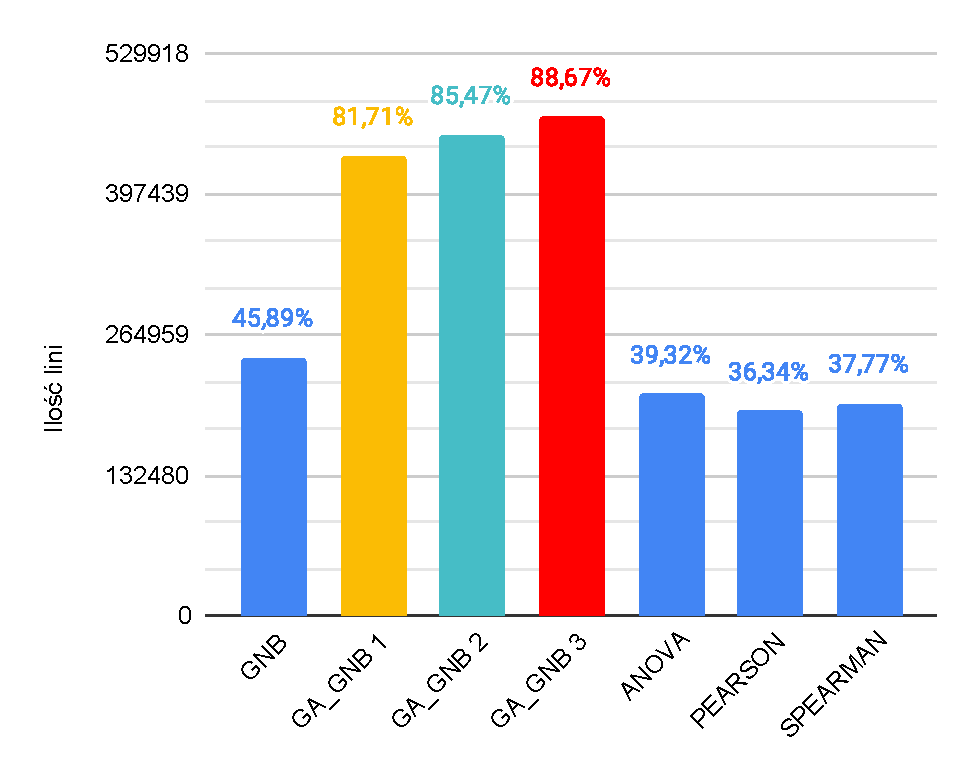
\includegraphics[width=0.7\textwidth]{images/Monday-WorkingHours_cmp}
    \captionsource{Klasyfikacja zbioru danych: Monday-WorkingHours}{\cite{Blyszcz2022}}
    \label{fig:mond}
\end{figure}

Analizując powyższe wyniki można zauważyć, że najwyższe dopasowanie uzyskał autorski algorytm a najniższe - zbiór kolumn wyznaczonych metodą współczynników korelacji Pearsona.\ Świadczy to o wysokiej jakości, opracowanego w pracy inżynierskiej, algorytmu.

